% This must be in the first 5 lines to tell arXiv to use pdfLaTeX, which is strongly recommended.
\pdfoutput=1
% In particular, the hyperref package requires pdfLaTeX in order to break URLs across lines.

\documentclass[11pt]{article}

% Remove the "review" option to generate the final version.
\usepackage[]{acl}

% Standard package includes
\usepackage{natbib}
\usepackage{lastpage}
\usepackage{fancyhdr}
\usepackage{times}
\usepackage{latexsym}
\usepackage{float}
\usepackage{graphicx}

% For proper rendering and hyphenation of words containing Latin characters (including in bib files)
\usepackage[T1]{fontenc}
% For Vietnamese characters
% \usepackage[T5]{fontenc}
% See https://www.latex-project.org/help/documentation/encguide.pdf for other character sets

% This assumes your files are encoded as UTF8
\usepackage[utf8]{inputenc}

% This is not strictly necessary, and may be commented out,
% but it will improve the layout of the manuscript,
% and will typically save some space.
\usepackage{microtype}

\pagestyle{fancy}
\fancyhead{}
\renewcommand{\headrulewidth}{0pt}
\fancyfoot[C]{Page \thepage \hspace{1pt} of \pageref{LastPage}}

% If the title and author information does not fit in the area allocated, uncomment the following
%
%\setlength\titlebox{<dim>}
%
% and set <dim> to something 5cm or larger.

\title{Detecting AI-Generated Images using ResNet}

\author{Ziyang Zeng \and Zhehu Yuan \and Yifan Jin \\
  Dept. of Computer Science \\
  New York University \\
  251 Mercer Street, New York, NY \\
  \texttt{zz2960@nyu.edu, zy2262@nyu.edu, yj2063@nyu.edu}}

\begin{document}
\maketitle
\begin{abstract}
  Recent advances in diffusion models have set an impressive milestone in image-to-image generation tasks. Trending works such as DALL-E2 and Stable Diffusion have attracted great interest in academia and industry. However, there are lack of evaluation about the images generated by these methods. In this paper, we generate synthetic images with the "Stable Diffusion" image diffusion generation model. The mixed dataset is mixed with the synthetic images and the original images and used as training data and test data in machine learning applications to investigate the capabilities of the Stable Diffusion model. Analyses show that the model training with ResNet could distinguish between the synthetic images and the original images with very high accuracy.
\end{abstract}

\section{Introduction}

Introduction goes here.


\section{Related Work}

Related work goes here.

\section{Datasets}

In order to train a classifier that can distinguish between real and generated images, we built a labeled dataset that consists of both real and generated images for supervised learning. Datasets of this kind is not common, and we'd like to experiment on the latest state-of-the-art image generation AI models, such as DALL·E 2 and Stable Diffusion. We started with real photos from existing public datasets as our raw datasets. Then, we use Diffusers-based image-to-image model to generate image variations from real photos. This way, we can get a labeled dataset that consists of both real and generated images.

\subsection{Raw Datasets}
\label{sec:raw_datasets}

The original real-world photos we experimented with are from public datasets: Indoor Scene Recognition Database and Weather Image Recognition Dataset. Additionally, we want to test how well our model performs on non-photo art work. A dataset that consists of pages of comic art (the Comic Books Images Dataset) is also used in our experiments.

\subsubsection{Indoor Scene Recognition Dataset}
\label{sec:indoor_dataset}

Originally targeting at indoor scene recognition tasks, the Indoor Scene Recognition Database is a collection of 67 indoor categories (e.g. airport, living room, restaurant...) and at least 100 images per category \cite{quattoni2009recognizing}. There are 15,620 images in the dataset in total. Figure \ref{fig:paper_indoor_dataset} shows some examples of the dataset.

\begin{figure}[h]
  \centering
  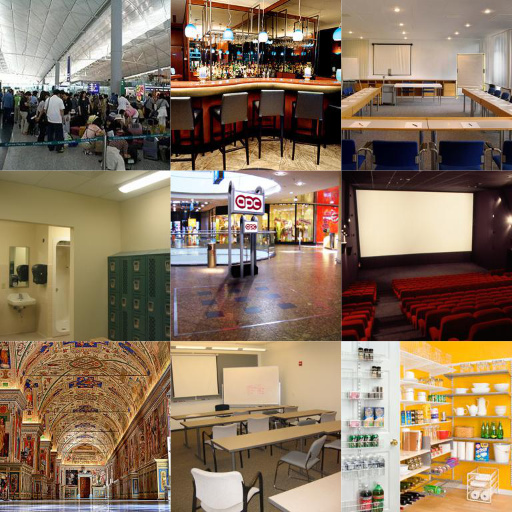
\includegraphics[width=140pt]{./assets/paper_indoor_dataset.jpg}
  \caption{Indoor Scene Recognition Database Examples}
  \label{fig:paper_indoor_dataset}
\end{figure}

This dataset is the biggest among the three datasets we used and serves as our main dataset. We use the AI-generated variations from these images and the images themselves to train our classifier.

\subsubsection{Weather Image Recognition Dataset}
\label{sec:weather_dataset}

The Weather Image Recognition Dataset contains labeled 6738 images of different types of weather, its catogories including dew, fog, frost, glaze, etc \cite{DVN/M8JQCR_2021}. This dataset is used in our experiment to evaluate our model's generalization ability and performance on other kinds of photos than indoors.

\begin{figure}[h]
  \centering
  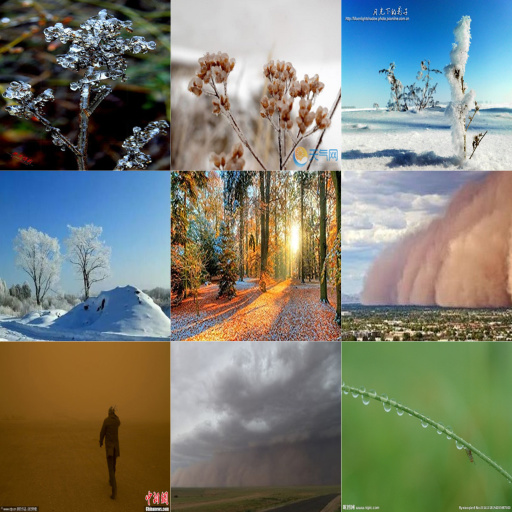
\includegraphics[width=140pt]{./assets/paper_weather_dataset.jpg}
  \caption{Weather Image Recognition Dataset Examples}
  \label{fig:paper_weather_dataset}
\end{figure}

\subsubsection{Comic Books Images Dataset}
\label{sec:comic_dataset}

The Comic Books Images Dataset is an open source dataset from Kaggle that contains 512 images from comic book pages \cite{cenkbircanoglu2017comicbooksimages}. Although our goal is to build a classifier to detect AI-generated photos versus real photos, and comic art seems to fall in neither category, we want to test whether our model can detect AI-generated comic art verses real comic art. This can further verify the generalization of our model. We what use to evaluation is a subset of this dataset, containing 513 images. Figure \ref{fig:paper_comic_dataset} shows some examples of the dataset.

\begin{figure}[h]
  \centering
  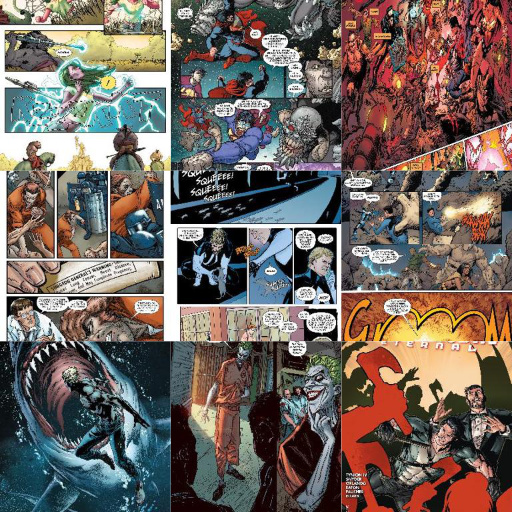
\includegraphics[width=140pt]{./assets/paper_comic_dataset.jpg}
  \caption{Comic Books Images Dataset Examples}
  \label{fig:paper_comic_dataset}
\end{figure}

\subsection{Image-to-Image Generation with Diffusers}

Instead of directly training on AI-generated images collected online, and compare them with the real photos from Section \ref{sec:raw_datasets}, we used an image-to-image (image-conditioned) generation pipeline to create AI-generated images from the real photos. The reason is that we think if we cannot make sure the AI-generated images and the real photos share the same themes, styles, content or objects, the model we train could learn that a certain theme/style of pictures containing certain things are from AI or real world without actually learning the general characteristics of the AI-generated photos. To mitigate this bias in the dataset, we came up with the solution of generating variations from given real world photos, so that our AI-generated images are of the same theme, similar style and content.

Even though diffuser-based image generation models have shown great success recently and achieved state-of-the-art results in conditioned image generation benchmarks, most of them are text-conditional, which means they take texts as an input to describe the images for the model to generate. In order for us to generate new variations of given real-world photos, we utilized an image-to-image generation pipeline that is present in DALL·E 2 APIs and a similar pipeline developed by Stable Diffusion community, which utilized image encoder output as conditioning.

\textbf{Diffusion models}, also known as DMs, are a type of generative model that sequenctially uses denoising autoencoders to synthesize new images. By decomposing the image generation process into a series of denoising steps, diffusion models can produce high-quality images that are similar to the ones they were trained on. To generate a new image, a diffusion model takes a noisy image as input, and starts with a certain step number. Then instead of directly predicting the denoised image, it uses denoising autoencoders to predict the noise added in the previous step, and then subtract that noise from the noisy image to get a less noisy image, because noise here is mathematically easier for the model to learn to predict. Then the slightly denoised image with a new step number that is smaller by 1 is fed into the autoencoder again to continue the denoising process. This process repeats until reaching step 1 where we have our final image.

\subsubsection{CLIP guidance}

CLIP (Contrastive Language-Image Pre-Training) is a neural network that has been trained on a large collection of (image, text) pairs. It has both an image encoder and a text encoder, and the goal of the model is to learn a representation of the images and texts that maximizes the cosine similarity between the representations of matching pairs \cite{radford2021learning}. As a result, CLIP model gives a great way to encode texts into vectors as embeddings, which is used in diffusion models like DALL·E 2 and Stable Diffusion to guide the image generation process so that the generated images fit the given texts. For every step of the diffusion process, the text encoder output from the CLIP model is used as image embedding into the denoising autoencoder to guide it to clear up noise. That way, the generated images are more likely to fit the description of the given texts, when the texts are used as conditioning.

A similar approach is to use the image encoder output from the CLIP model as image embedding into the denoising autoencoder. This is the approach we used in our project. We used the image encoder output from the CLIP model as image embedding into the denoising autoencoder to guide it to clear up noise. This way, the model appears to generate variations of the given image that are similar to the them.

\subsubsection{Stable Diffusion}

Stable Diffusion is one of the recent text-to-image models released in 2022 and is a latent diffusion model, a variety of deep generative neural network developed by the CompVis group at LMU Munich \cite{rombach2022high}. It combines the advantages of powerful pretrained autoencoders and diffusion models, which are sequential applications of denoising autoencoders, to achieve state-of-the-art synthesis results on image data and beyond. Since Stable Diffusion is the only open-source one among the 3 most popular diffusion models and it is designed to reduce computational requirements while retaining visual fidelity can run on most consumer hardware equipped with a modest GPU, we can run it on Google Colab to generate part of our main dataset while paying no licensing fee for the model.

\subsubsection{DALL·E 2}

DALL·E 2, on the other hand, is a similar text-to-image generative model that also uses a diffusion model conditioned on CLIP image embeddings, and is developed by OpenAI as commercial product providing inference API services \cite{ramesh2022hierarchical}. DALL·E 2 is trained on a large collection of proprietary captioned high-quality stock images other than scraped images from the internet like Stable Diffusion. As a result, DALL·E 2 is capable of generating more intricate and sophisticated images than Stable Diffusion or Midjourney, which is another closed-source Diffusion model that is more known for its artistic style \cite{oppenlaender2022creativity}. DALL·E 2 comes with a image variation generation API which, under the hood, uses the image encoder from CLIP to condition the diffusion model, similar to what we use with Stable Diffusion. Because of our limited budget, we cannot afford to use DALL·E 2 to generate our main dataset, but we can use it to generate two small datasets for validation.

\subsubsection{Image Variation Generation}
\label{sec:datasets_image_variation_generation}

As mentioned, we want to generate variations of the given real-world photos from our raw datasets, and then label both the generated images and the original real-world photos together to build a dataset for training our AI-generated image binary classification model. Our main generative model choice is Stable Diffusion since it's open-source and has a relatively small memory footprint.

Stable Diffusion is originally trained to be a text-to-image model, which means it takes texts as input to describe the images for the model to generate. In order for us to use it as an image-to-image model, we use a pipeline that is similar but swaps the text encoder with the image encoder from CLIP. Since the goal for training CLIP is to maximize the cosine similarities for the image presentation by the image encoder and the text presentation by the text encoder for matching (image, text) pairs, after the CLIP has been trained, the output presentations (vectors) from it for matching text and image are very similar, thus the swapped-in image encoder in the Stable Diffusion model we use could play the same role of guiding the diffusion model to generate images similar to the input images. The image encoder from CLIP is used to encode the image into a vector, which is then used as image embedding into the diffusion model to guide it during denoising steps, similar to DALL·E 2's image variation generation API. This way, the model appears to generate variations of the given image that are similar to the them.

\subsection{Processed Datasets}

By running CLIP-image-encoder-guided Stable Diffusion mentioned in Section \ref{sec:datasets_image_variation_generation} on our raw datasets, we built our main dataset from the indoor dataset in Section \ref{sec:indoor_dataset} which contains 15,621 real-world in-door photos and combined with another 15,621 generated images that are similar to the real-world photos. Aside from the main dataset, we also built two smaller datasets from the weather dataset in \ref{sec:weather_dataset} and the comic book dataset in \ref{sec:comic_dataset} for testing the model's generalization on other genres of photos. For each image in this dataset, we applied center-cropping and resizing postprocessing to make sure they are consistent in image size, being 256x256.


\section{ResNet Classifier}

The main task of this project is classification. Over the years, researchers tend to make deeper neural networks(adding more layers) to solve such complex tasks and to also improve the classification accuracy. But, it has been seen that as we go adding on more layers to the neural network, it becomes difficult to train them and the accuracy starts saturating and then degrades also. Therefore, we decided to use \textbf{ResNet}, which overcomes the above issue, to do the classification.

ResNet, short for Residual Network, provides another way for data to reach later regions of the neural network by skipping some layers. Consider a series of layers, from layer $I$ to layer $I + n$, and the function $F$ that these layers represent. Layer $i$'s input is denoted by $x$. $x$ will simply run through these layers one by one in a classic feedforward arrangement, and the result of layer $I + n$ is $F(x)$$.

The Resnet conducts element-wise addition $F(x) + x$ after applying identity mapping to $x$. A residual block or a building block is the term used in literature to describe the entire architecture that takes an input $x$ and creates an output $F(x) + x$. An activation function, such as ReLU applied to $F(x) + x$, is frequently included in a residual block.

The advantage of adding this type of skip connection is that if any layer hurt the performance of architecture then it will be skipped by regularization. So, this results in training a very deep neural network without the problems caused by vanishing/exploding gradient.The training process of a neural network with residual connections has been proven to converge significantly more readily.


\section{Experiments}



\subsection{Experiment Settings}

As discussed in the previous section, the classification model is Resnet34 integrated inside the fastai. About the dataset:

\subsubsection{Training}

We split around 80\% of the Indoor Scene Recognition Dataset with its generated pictures (using Stable Diffusion) for the training part.

\subsubsection{Validation}

We split around 20\% of the Indoor Scene Recognition Dataset with its generated pictures (using Stable Diffusion) for the validation part. The validation data is not used in the training process.

\subsubsection{Testing}

The testing dataset includes several types of pictures:

\textbf{Stable Diffusion model:} In order to test the generalization ability of our Resnet34 model and to verify it really learns the features of Stable Diffusion generation, not any specific features of Indoor pictures, we use the same method to generate the following dataset which has different pictures contents than Indoor Scene Recognition Dataset:

(1) Weather Image Recognition Dataset: real-world weather pictures with generated pictures.

(2) Comic Books Images Dataset: comic book images with generated pictures.

\textbf{Dalle2 model: } Besides, we want to test whether the model can distinguish AI pictures generated by other methods. Thus, we choose the same Weather Image Recognition Dataset but generate AI picutres using Dalle2 model to test the performance.

\subsection{Evaluation Metrics}

To evaluate the performance of the model, we used accuracy, precision, recall and F1-score as evaluation metrics. Below are the formulas for calculating the accuracy, precision, recall and F1-score. Here we assume the AI-generated pictures as positive labels while original pictures as negative labels. Thus, TP is the number of AI pictures being correctly predicted as AI pictures, FP is the number of original pictures being wrongly predicted as AI pictures. Similarly, TN is the number of original pictures being correctly predicted as original pictures, FN is the number of AI pictures being wrongly predicted as original pictures.

\[
Accuracy = \frac{TP+TN}{TP+FP+TN+FN}
\]
\[
Precision = \frac{TP}{TP+FP}
\]
\[
Recall = \frac{TP}{TP+FN}
\]
\[
F1 = \frac{2 \times Precision \times Recall}{Precision + Recall}
\]


\section{Experiment Results}

Experiment results go here.

\begin{figure}[htbp]
\centering
\subfigure{
\begin{minipage}[t]{\linewidth}
\centering
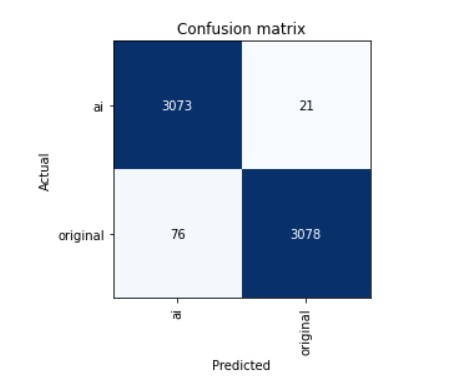
\includegraphics[width=4in]{paper/training_confusion_matrix.jpg}
\caption{Validation Confusion Matrix}
\end{minipage}%
}%
\end{figure}

\section{Conclusion}

Conclusion goes here.

\section{Discussion and Future Work}

Discussion and future work go here.

% \printbibliography
\bibliographystyle{plain}
\bibliography{refs}

\end{document}
